\RequirePackage[l2tabu, orthodox]{nag}
\documentclass[a4paper,11pt]{scrreprt}

\def\Author{Andreas Bock, bock@andreasbock.dk\\
Johan Astborg, joastbg@gmail.com\\\\
Supervisors:\\
Jost Berthold, jb.diku@gmail.com\\
Sinan Gabel, sinan.gabel@gmail.com
}
\def\Title{\bf HQL - \textsc{Hiperfit} Quant Library\\ {\Large Project Report}}

%
%--------------------   start of the 'preamble'
%

\usepackage{tikz}
\usepackage{graphicx,amssymb,amstext,amsmath,graphics,epsfig,color}
\usepackage{fancyhdr}
\usepackage[toc]{glossaries}
%\usepackage{algorithm}
%\usepackage{algorithmic}
%\usepackage{lmodern,inconsolata}
\usepackage{array, xcolor, lipsum, bibentry, fancyhdr}
\usepackage[absolute]{textpos}
%\usepackage[top=25mm, bottom=25mm, left=22mm, right=22mm]{geometry} %Layout of page
\usepackage{lastpage} % number of last page 
\usepackage{hyperref}
\usepackage{lipsum}
\usepackage{microtype}
\usepackage{ctable}
\usepackage{tikz}
\usepackage{listings,setspace,framed}
\usepackage{minted}
%\usepackage[toc, section, numberline,acronym]{glossaries}
%\usepackage[toc, section, numberline,acronym]{glossaries}

\usepackage{makeidx}
\usepackage[intoc]{nomencl}


%\usepackage[toc,acronym]{glossaries} 

\makeindex 
\makeglossaries

%
%%    homebrew commands -- to save typing
\newcommand\etc{\textsl{etc}}
\newcommand\eg{\textsl{eg.}\ }
\newcommand\etal{\textsl{et al.}}
\newcommand\Quote[1]{\lq\textsl{#1}\rq}
\newcommand\fr[2]{{\textstyle\frac{#1}{#2}}}
\newcommand\miktex{\textsl{MikTeX}}
\newcommand\comp{\textsl{The Companion}}
\newcommand\nss{\textsl{Not so Short}}
\renewcommand{\bibname}{References}
\makeglossaries

% Comments
\newcommand{\comm}[2]{{\sf \(\spadesuit\){\bf #1: }{\rm \sf #2}\(\spadesuit\)}}
\newcommand{\mcomm}[2]{\marginpar{\scriptsize \comm{#1}{#2}}}
\newcommand{\ab}[1]{\mcomm{AB}{#1}}
\newcommand{\ja}[1]{\mcomm{JA}{#1}}

%% Glossaries
\usepackage[T1]{fontenc} % font
\setlength{\parindent}{0in}
\definecolor{lightgray}{rgb}{0.9,0.9,0.9}

\newenvironment{filecode}[1][]
{\minipage{\linewidth}
\lstset{basicstyle=\ttfamily\footnotesize,frame=single,
numberstyle=\small\color{black},keywordstyle=\color{black},commentstyle=\color{black},
stringstyle=\color{black},tabsize=2,backgroundcolor=\color{lightgray},language=Haskell,#1}}
{\endminipage}
\renewcommand*\rmdefault{ppl}

%\pagestyle{fancy}
%\fancyhf{} 
 
%\lhead{\uppercase{Hiperfit Quant Library}}
%\rhead{\nouppercase{\rightmark}}
 
\cfoot{\thepage}
 
\lfoot{
\begin{textblock*}{100mm}(30mm, 280mm )
\end{textblock*}
}

%
%---------------------   end of the 'preamble'
%
\newcommand{\HRule}{\rule{\linewidth}{0.5mm}}

\pagestyle{fancy}               % Fräcka sidhuvuden
%\addtolength{\headwidth}{2cm}   % Sidhuvd bredare än texten.
\renewcommand{\headrulewidth}{0.4pt} % Linje i sidhuvud är 0.4 punkter
%\renewcommand{\footrulewidth}{0.4pt} % Linje i sidfot är 2 punkter

% Följande kommandon definerar vad som ska finnas i sidhuvud och
% sidfot. Om man skriver dubbelsidiga dokument anger man två alternativ
% med komma mellan. Den första gäller då för udda sidor och den andra
% för jämna sidor. Bokstäverna ska tolkas som:
% L = left, C = center, R = right,
% E = even (jämna sidor), O = odd (udda sidor)
% E och O fyller ingen funktion om man inte har optionen twopage definierad
\fancyhead[R]{\bf{\nouppercase{\leftmark}}}	% Vänstertext i sidhuvud
\fancyhead[L]{\nouppercase{\rightmark}}	% Högertext i sidhuvud
%\fancyfoot[C]{}	% Mittentext i sidfot
%\fancyfoot[LO,RE]{}		% Vänster udda, höger jämna sidor
%\fancyfoot[LE,RO]{}	% Vänster jämna, höger udda sidor


%%%%********************************************************************
% fancy quotes
\definecolor{quotemark}{gray}{0.7}
\makeatletter
\def\fquote{%
    \@ifnextchar[{\fquote@i}{\fquote@i[]}%]
           }%
\def\fquote@i[#1]{%
    \def\tempa{#1}%
    \@ifnextchar[{\fquote@ii}{\fquote@ii[]}%]
                 }%
\def\fquote@ii[#1]{%
    \def\tempb{#1}%
    \@ifnextchar[{\fquote@iii}{\fquote@iii[]}%]
                      }%
\def\fquote@iii[#1]{%
    \def\tempc{#1}%
    \vspace{1em}%
    \noindent%
    \begin{list}{}{%
         \setlength{\leftmargin}{0.1\textwidth}%
         \setlength{\rightmargin}{0.1\textwidth}%
                  }%
         \item[]%
         \begin{picture}(0,0)%
         \put(-15,-5){\makebox(0,0){\scalebox{3}{\textcolor{quotemark}{``}}}}%
         \end{picture}%
         \begingroup\itshape}%
 %%%%********************************************************************
 \def\endfquote{%
 \endgroup\par%
 \makebox[0pt][l]{%
 \hspace{0.8\textwidth}%
 \begin{picture}(0,0)(0,0)%
 \put(15,15){\makebox(0,0){%
 \scalebox{3}{\color{quotemark}''}}}%
 \end{picture}}%
 \ifx\tempa\empty%
 \else%
    \ifx\tempc\empty%
       \hfill\rule{100pt}{0.5pt}\\\mbox{}\hfill\tempa,\ \emph{\tempb}%
   \else%
       \hfill\rule{100pt}{0.5pt}\\\mbox{}\hfill\tempa,\ \emph{\tempb},\ \tempc%
   \fi\fi\par%
   \vspace{0.5em}%
 \end{list}%
 }%
 \makeatother
 %%%%********************************************************************

%-----------------------------------------------------------
%% Has to be defined before begin/document

%% Use separate latex file for this...

\newglossaryentry{bar}{name={bar}, description={\ldots}}
\newglossaryentry{baz}{name={baz}, description={\ldots}}

\newacronym{foobar}{foobar}{\ldots}
%-----------------------------------------------------------

\begin{document}

%-----------------------------------------------------------
\begin{titlepage}

\textsc{\LARGE }\\[1.5cm]
\textsc{\Large }\\[0.5cm]
\textsc{\large }\\[0.5cm]
 
% Title
\begin{center}
\HRule \\[0.5cm]
\huge \bfseries \Title\\[0.5cm]
\HRule \\[0.5cm]

% Author
\Large
%\emph{Authors:}\\
\textsc{Andreas Bock \\ Johan Astborg }\\[3cm]


\date{\today}



% Bottom of the page
{\today}\\[4cm]
%\includegraphics{Logo}\\[1cm] % Department/University logo
 
\vfill
\end{center}

\end{titlepage}
%-----------------------------------------------------------
\begin{abstract}

We present our project, \textsc{Hiperfit} Quant Library, where we design and develop the architecture for a Haskell library for quantitative finance.

\end{abstract}
%-----------------------------------------------------------
\tableofcontents
%-----------------------------------------------------------
\listoftables
\addcontentsline{toc}{chapter}{List of Figures}
\listoffigures

%\printglossary

%-----------------------------------------------------------

\chapter{Introduction}

Our lives becoming increasingly dependent on IT, and as a result, software errors are manifold. The financial sector has a particular low tolerance, as erroneous software may have dire consequences in the form of massive monetary loss.
The financial crisis of 2008 also caused legislators to take a conservative
stance on risk (cite), as the collapse on Lehman Brothers reverberated throughout the world's economies.
Consequently, financial institutions' risk management tools must become more sophisticated, putting stress on the quality of the software.

We present a prototype Haskell library for valuation of financial products.

The project was conducted within the \textsc{Hiperfit} research center at the
University of Copenhagen.

Lorem ipsum \gls{bar} \gls{baz} and \gls{foobar}.

\cite{Borman03raytracingand}
\chapter{Background}

A financial security is a legal claim on a firm's asset or income 
that is traded in an organized market\cite{alexander2008market}.
A portfolio is  a number of positions in such securities, equities, bonds
and other types of financial instruments. 
Such instruments are typically traded on an exchange such as 
\href{http://www.nasdaqomxnordic.com/}{NASDAQ OMX Nordic}, but so-called
\emph{over-the-counter} (OTC) products also exist where two parties enter
a unilateral, legally binding, trade.\\
The value of such a collection can be computed to reflect the theoretical 
value they would have if they existed today to allow investors to assess
whether resources could yield higher returns elsewhere.\\
Financial instruments are priced differently, some using closed-form functions 
and others relying on stochastic simulation. The former plays a large part in
our project, while the latter is scoped out.\\

Such analyses involve an understanding of the industries in question,
economics, mathematics and computer science. For instance,
domain-specific knowledge in the energy 
industry is a prerequisite for fruitful investing in oil. Similarly, economists 
must apply their knowledge to best assess market trends and constantly reevaluate
the forecasts they base their trading on.
Further, people known as \emph{quants} combine mathematics and computer science
in creating and implementing models for risk management, asset pricing or 
algorithmic trading.\\
In this project we seek to coalesce mathematical finance and software engineering
into a software tool set employed by \emph{quants}.\\

There exist two pivotal components that are key to the pricing of assets in the
fixed income category. The first is discounting which is a method of scaling
future cashflow so as to represent its  theoretical value it would have had
it existed today.
As the prevailing interest rate is observable, the time value of money enables 
the investor to assess whether an investment is up to par. A promise of a 
payment in the future therefore has to be proportional to what the investor 
otherwise would have been able to receive in the market.\\

Secondly is credit risk is a method of evaluating the creditworthiness of a 
debitor, i.e. quantifying how likely it is that the counterpart will pay back 
its debt. This  is not considered for exchange-traded products, as losses 
caused by defaults 
are covered by the members of the exchange\footnote{If a large exchange 
defaults the world economy would be in utter turmoil.}. However, for OTC
products, the evaluation of credit risk is critical as the consequences of a 
default of the counterparty lies solely with the opposing party. Since the 
financial crisis of 2008 this has become increasingly important for financial 
institutions, and \href{http://www.lchclearnet.com/}{clearing houses} have
been established to mitigate the 
domino effect of collapses of large financial institutions.
The time value of money and credit risk are two key components allowing 
investors to gauge whether an investment will be in their favour.\\

\section{Related work}

In terms of free software, the amount of quantitative finance libraries is 
limited.
The most prominent is Quantlib, an open-source C++ library\cite{Ame2003}
supporting a wide array of financial products ranging from bonds to more 
exotic derivatives.\\

Hquantlib\cite{hquantlib} is an attempt at a Haskell port of Quantlib
and is under 
development.\\

Peyton Jones and Eber\cite{composingcontracts} developed a combinator library 
allowing users to define virtually any financial contract by means of a
computational denotational semantics.
\ab{Should this be more explicit?}

Sinan Gabel developed DerivativesExpert\cite{Mathematica:DerivativesExpert}
, an extension for \href{http://www.wolfram.com/mathematica/}{Mathematica}
for valuation of financial products such as bonds, interest rate derivatives 
and options. Our project aims to create the core Haskell architecture for 
valuation of such products and re-engineer a subset of DerivativesExpert, 
(mainly fixed income securities) into Haskell.

\chapter{Fixed Income}
 \begin{fquote}[John von Neumann][1903-1957]If people do not believe that mathematics is simple, it is only because they do not realize how complicated life is.
 \end{fquote}

This document will describe in detail the building blocks of a modern high performance ray tracer.
Feature list:
\begin{itemize}
\item Choice of Language, C++
\item Basic Whitted ray-tracing
\item Kd-Tree acceleration structure
\end{itemize}
Cras nisi neque, pharetra ac cursus nec, vestibulum sit amet erat. Vivamus eget viverra elit. Sed vehicula augue sit amet nibh convallis volutpat. Sed feugiat posuere nunc a auctor. Nam turpis erat, ultrices sed varius in, tempus nec enim. Donec hendrerit dignissim libero, non lacinia odio congue non. Nulla eu velit urna, ut accumsan nibh. Fusce ligula massa, volutpat ut blandit at, dignissim sed orci. Nulla sed mauris lorem. Mauris nec turpis purus, sed sollicitudin massa. Sed ipsum purus, vestibulum et viverra et, tristique at leo. Cum sociis natoque penatibus et magnis dis parturient montes, nascetur ridiculus mus. Sed gravida, odio a rutrum posuere, diam erat fermentum arcu, sit amet blandit orci metus ac mauris.

\chapter{Key Concepts and Architecture}

In this section we will go through the architecture of HQL and describe how we
modelled the various of financial instruments in Haskell. We shall introduce
the necessary mathematical finance and conventions as we go along.

\section{Language features}

Functional languages lend themselves well to the domain of finance due
to several reasons such as modularity\cite{hughes:matters-cj}, 
laziness\cite{composingcontracts}. Moveover, the mathematical
 nature of finance makes functional languages suitable for valuation due its
inherent mathematical foundation and purity.\\

Haskell's advanced type system eliminate a whole class of bugs related to 
type errors and its 
class system allows us to define type-safe interfaces for operations on 
financial products who themselves can be represented by Haskell data types. 
Statically typed languages have the advantage of discovering a multitude of
errors at compile time, and the type class system enables us to overload 
functionality in our programs based on our types. This is a very desirable
feature, as we want our financial products to have the same API (e.g. a function 
called \texttt{presentValue} should return the present value regardless of the
product type).\\

Figure \ref{fig:overview} shows an overview of the entities we are dealing with
and situaion we wish to model. Ultimately, each item in this figure must somehow
be represented in Haskell using a class or type depending on the the item.

We want to model a library that features financial products, mathematical models
for valutation and finally what we call a pricing engine, which combines the 
these contracts and mathematical models with the current state of the world
in order to produce meaningful measurements of said contract.\\

\begin{figure}[h!]
\begin{center}
\begin{minipage}{\linewidth}
\makebox[\linewidth]{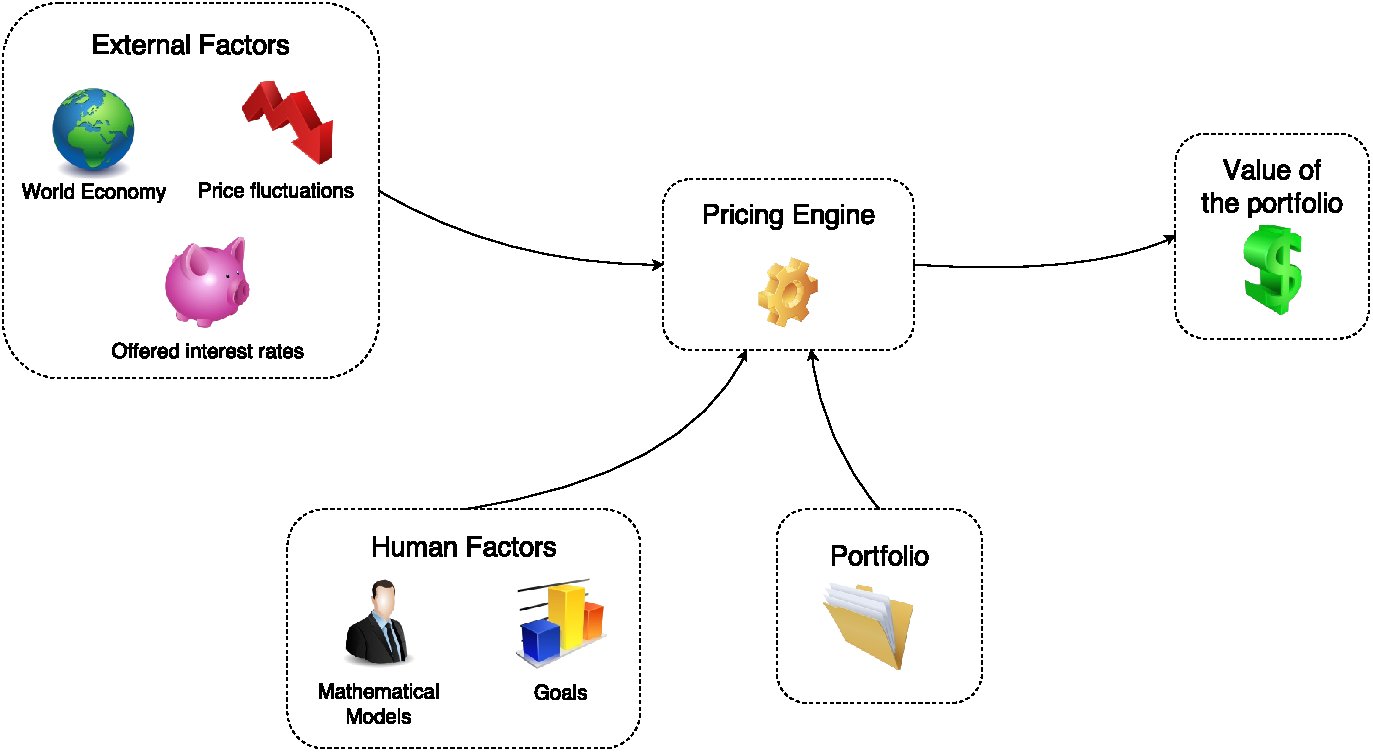
\includegraphics[keepaspectratio=true,scale=0.6]{images/Overview.pdf}}
\caption{Overview of what we want to model.}
\label{fig:overview}
\end{minipage}
\end{center}
\end{figure}

We shall begin with the modelling aspects and provide the reader with the
matematical finance required. Thereafter we will present the contracts, and
finally how such a pricing engine is modelled. 

\section{Interest Rates}

We begin our introduction to mathematical finance with a concept familiar to
most, name interest rates. An interest rate is the the amount of return on
investing an amount of money for a set amount of time. This can be formulated
using a very simple equation, which we will demonstrate with a one year flat
interest rate on a deposits account:

\begin{equation}\label{eq:lincomp}
FV_T = N (1 + R_T)
\end{equation}

where $FV_T$ denotes the future value in $T=1$ periods, $N$ is the principal
and $R_T$ is the rate over the period $T$\footnote{$T$ is also referred to as the
\emph{tenor}.}. Extending this to multiple years we introduce a new 
concept called compound interest, which is simply the formula above reapplied
a number of times. The intuitive approach is
that the compound interest is the return from reinvesting previously invested
capital. Mathematically, this return can be formulated as an exponentially 
compounded interest rate:

\begin{equation}\label{eq:expcomp}
FV_{T_n} = N (1 + R_{T_n})^n
\end{equation}

where $FV$ is now dependent on the number of times it is compounded, and is 
therefore also called periodic compounding.
While this model is easy to understand, the world of finance demands much more 
intricate details to correctly understand it. First, it assumes 
discrete time periods, but we have not specified if this $n$ stands for days, 
months, or years, or how what the tenor is. Further, it assumes that compounding
occurs at after every period, which is not necessarily so. For instance, the
equation \ref{eq:expcomp2} with $n=1$ and $m=2$ describes the return on a one-year
investment with semiannual compounding:

\begin{equation}\label{eq:expcomp2}
FV_{T_n}^{n,m} = N (1 + \frac{R_T}{m})^{mn}
\end{equation}

does not  All of these intricacies are critical for correctness of \hql and must
be accounted for in the implementation.\\

Up until this point we have assumed that the compounding is performed at 
discrete intervals. However, as \ref{eq:expcomp} is simply a formula, we may apply 
methods  from calculus to achieve what is known as the continuously compounded interest 
rate. It is defined as the resulting interest rate when we take the limit of 
equation \ref{eq:expcomp} as $n$ goes to infinity:

\begin{equation}
\text{lim}_{n \rightarrow \infty}\; FV_T^n \; = \text{lim}_{n \rightarrow \infty}\; N (1 + R_T)^n
= N e^{RT}
\end{equation}

where $R$ is the continuously compounded interest rate. This rate is much easier
to work with in advanced fixed income modelling\cite{cmunk}, as we can disregard
the details concerning periods and compounding intervals. Further, it yields
sufficiently close numerical results.

\begin{figure}[!htb]
\centering
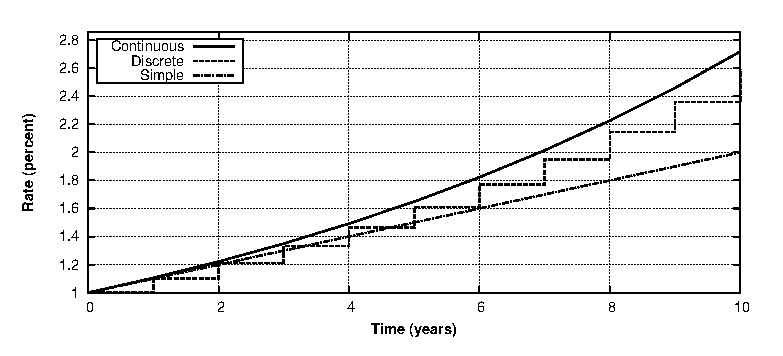
\includegraphics[scale=1.2]{images/comp02.eps}
\caption{How compounding methods influence returns.}
\label{fig:comp02}
\end{figure}

Figure \ref{fig:comp02} shows the influence in rate as a result of the different
kinds of compounding. Note that the return of the different compounding methods
diverges after the first year. Furthermore, table \ref{tab:cmptable} gives an 
overview of the relation between compounding functions and time steps.It should 
be evident to the reader that the notion of linear continuously compounded interest
rate is absurd, as we derive it from equation \ref{eq:expcomp}.

\begin{center}  
\begin{longtable}{|r|c|c|}
\hline  
\backslashbox{Time}{Compounding}
           &Linear\footnote{Also referred to as a \emph{simple} rate.} & Exponential\\\hline
Discrete   & Flat   & Periodic\\\hline
Continuous & \textcolor{red}{\xmark} & Continouous\\\hline
\caption{Compounding and time steps.}
\end{longtable}
\label{tab:cmptable}
\end{center}

We see that the method of compounding has very distinct impact on the returns.
From a modelling perspective, this means that we have designed Haskell
data types to distinguish between interest rates differing in the compound
method as follows:

\begin{hscode}
type Rate = Double
newtype ContinuousRate = ContinuousRate Rate deriving (Show)
newtype SimpleRate     = SimpleRate Rate deriving (Show)
data ExponentialRate   = ExponentialRate Rate Frequency deriving (Show)
\end{hscode}

The simplicity of the types come at the of the assumption that all rates are
annualized. This way, we only require a \texttt{Frequency} (an integer) to
denoting number of times interest is compounded per year in the
\texttt{ExponentialRate} type.\\
Using the Haskell type system we can make sure that a continuously compounded
rate is not mistakenly used in a function that expects a simple rate.
Note that \texttt{newtype} does not exacerbate overhead.\\

As we will see, it is often convenient to convert a rate such as the ones above
into equivalent a simple rate. We have therefore chosen to model an
\texttt{InterestRate} class that defines a number of methods, allowing for
abstraction of the underlying rate:

% TODO : Explain the Daycount convention + Calendar

\begin{hscode}
type Offset = Double -- offset from today in years
type Factor = Double
class InterestRate r where
  -- | Returns the corresponding continuously compounded rate
  continuousRate :: r -> ContinuousRate
  -- | Returns the discount factor at an offset
  discountFactor :: r -> Offset -> Factor 
  -- | Reciprocal of the discount factor
  compoundFactor :: r -> Offset -> Factor 
  -- | Get the intrinsic rate
  rate           :: r -> Rate
\end{hscode}

A central tenet of our architecture is that we keep the backend
as simple as possible and keep the interface detailed and 
self-explanatory. This way we keep the mathematical formulas as transparent
and clean as possible while the interface remains user-friendly. An example
of this is our use of the \texttt{Offset} type, which indicates a point in 
time relative to today, measured in years (e.g. an offset of $0.5$
means six months from today). The interface, which remains to be seen, uses
a somewhat convoluted Calendar module (due to several conventions in the 
financial world), however the pricing backend we are currently describing 
is completely oblivious to this fact.

Further, as we mentioned above, advanced fixed income modelling and options 
pricing often use the continuously compounded rates due to its mathematical 
properties\cite{HULL}. The \texttt{continuousRate} function caters to this
need, as it essentially solves the following equation for $R_C^n$:

\begin{equation}
e^{R_C^n} = (1+R_p)^n
\end{equation}

where is $R_p$ the exponentially (periodically) compounded rate.\\

The \texttt{discountFactor} function introduces concept that we
explain in the following section.

We refer to the \hql documentation\cite{hqldoc} for an in-depth treatment of the
mathematical finance pertaining to interest rates.

\section{Discounting}\label{sec:discounting}

We first present the basic theory of cashflow discounting, and motivate with
a small example. Given an option to invest an initial amount and receive 
\$$100$ in a year from now, how would you decide whether or not to invest? In
other words, what is the price of such an investment? If the investment bears
an interest rate of 5\%, then we may use equation \ref{eq:lincomp} to solve
for $N$, the initial investment i.e. the price:

\begin{equation}
100 = N (1 + 0.05) \Leftrightarrow N = \frac{100}{1+0.05}
\end{equation}

More generally, we have:

\begin{equation}
DF_T FV_T= N (1 + R_T)
\end{equation}

Therefore our discount factor, $DF_T$, is $\frac{1}{1.05} \approx 0.95238$,
so the \emph{present value} (or price) of the investment is \$$95.238$
in the example above. If we have other viable options to invest in over the coming
year, the decision becomes more complex.

Imagine a second party offering \$$90$ in one year with an additional payment of
\$$10$ after six months. Summing the two cashflows could make us believe that the
two options are equal. However, due to the time value of money, the latter option
is favourable. This is because we may reinvest the \$$10$ over the remaining six
month tenor of the investment! We present the scenario pictorially in figure
\ref{fig:tvom} below.

\begin{figure}[h!]
\begin{center}
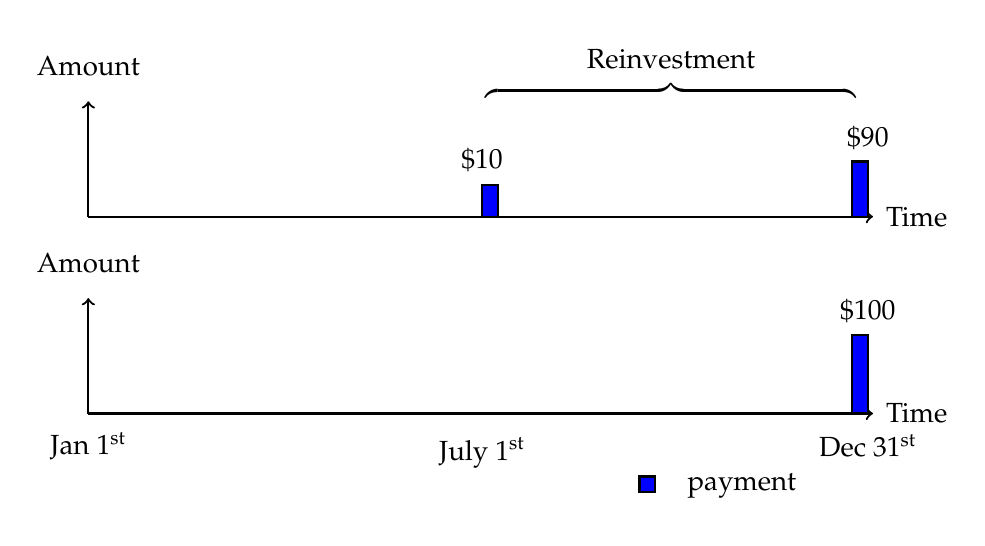
\begin{tikzpicture}[-,shorten >=1pt,auto,node distance=1.5cm,thick,minimum size=0.8cm,main node/.style={circle,draw=red,very thick}]
\tikzstyle{selected edge} = [draw,line width=6pt,-,blue!30]
\coordinate (belowstart) at (0,-1);

\coordinate (origo0) at (0,0);
\coordinate (xaxis0) at (10,0);
\coordinate (yaxis0) at (0,1.5);
\coordinate (face0s) at (9.9,0);
\coordinate (face0e) at (9.9,1.2);

\coordinate (origo1) at (0,2.5);
\coordinate (xaxis1) at (10,2.5);
\coordinate (yaxis1) at (0,4);
\coordinate (face1s) at (9.9,2.5);
\coordinate (face1e) at (9.9,3.3);

\coordinate (sixmpay1) at (5,2.5);
\coordinate (sixm1) at (5,2.80);

% Draw axes 0
\draw[->] (origo0) -- (xaxis0) node[right] {Time};
\draw[->] (origo0) -- (yaxis0) node[above] {Amount};

% Draw axes 1
\draw[->] (origo1) -- (xaxis1) node[right] {Time};
\draw[->] (origo1) -- (yaxis1) node[above] {Amount};
\draw[] (sixmpay1) -- (sixm1) node[above] {\$10};

% Draw reinvestment option
%\draw[dotted,draw=blue] (5.2,3.3) [bend left] (face1e);
\node[] at (7.4,4.1) {$\overbrace{\phantom{\hspace{4.7cm}}}$};
\node[] at (7.4,4.5) {Reinvestment};
\node[] at (5,-0.5) {July 1$^{\text{st}}$};

\filldraw[draw=black, fill=blue] (sixmpay1) rectangle node {} +(0.2,0.4);
\filldraw[draw=black, fill=blue] (9.7,2.5) rectangle node {} +(0.2,0.7);
\filldraw[draw=black, fill=blue] (9.7,0) rectangle node {} +(0.2,1);
%\filldraw[draw=black, fill=lightgray]  (10,1) rectangle node {} +(0.2,0.1);

% Legend
\filldraw[draw=black, fill=blue] (7,-1) rectangle node {} +(0.2,0.2);
\node at (8.3, -0.92) () {payment};
\node at (9.9,3.5) () {\$90};
\node at (9.9,1.3) () {\$100};

% "Legend"
\draw[] (origo0) -- (origo0) node[below] {Jan 1$^{\text{st}}$};
\draw[] (9.9,0) -- (9.9,0) node[below] {Dec 31$^{\text{st}}$};

\end{tikzpicture}
\caption{Two investment opportunities showing the time value of money.}
\label{fig:tvom}
\end{center}
\end{figure}

As investors want to maximize profits, it is quite intuitive to think that
the decision to invest directly depends on what alternatives are available.
Assuming resources are limited, it may quickly become difficult to asses which
option is opportune if the market offers multiple choices. As the discount factor
is just the inverse of the interest rate, \texttt{discountFactor} is part of the
interface for interest rates.\\

Again we refer the reader to the documentation\cite{hqldoc} for examples of
how this is done in \hql.\\

Since we must consider all options to maximize our profits, we must somehow have an
overview of the interest rates currently offered in the market. This leads us onto the
next key element in pricing theory, namely the term structure of interest rates.

\section{Term Structure}

A term structure can be viewed as a function f that given a tenor returns 
an interest rate. Since these are zero rates, term structures are valuable 
tools in finance as we may use them to discount any cashflow regardless how it
was generated.

\ab{What do}
%The converse is not true, we cannot use the rate over the tenor
%of a serial to discount a future income stream, unless that follows the exact
%same cash flow pattern.\\

\begin{figure}[h!]
\begin{center}
\begin{tikzpicture}[-,shorten >=1pt,auto,node distance=1.5cm,thick,minimum size=0.8cm,main node/.style={circle,draw=red,very thick}]
\tikzstyle{selected edge} = [draw,line width=6pt,-,blue!30]
\coordinate (belowstart) at (0,-1);
\coordinate (xaxis) at (10,0);
\coordinate (origo) at (0,0);
\coordinate (yaxis) at (0,5);

% Draw axes
\draw[->] (origo) -- (xaxis) node[right] {Time to maturity};
\draw[->] (origo) -- (yaxis) node[above] {Annual rate};

% Flat TS
%\draw[thick,draw=blue] (0,1.5) -- (10,1.5);
% "Normal" TS
\draw[thick,draw=green] (0,0) parabola[bend at end] (10,5);
% Inverse TS
%\draw[thick,draw=red] (0,5) parabola[bend at end] (10,0.5);

\draw[dotted] (3,2.53) -- (3,0) node[below] {\text{ 3.5 years}};
\draw[dotted] (3,2.53) -- (0,2.53) node[left] {2.4\%};

% Legend
%\filldraw[draw=black, fill=blue] (5.2,-1) rectangle node {} +(0.2,0.2);
%\node at (6, -0.92) () {Flat};

%\filldraw[draw=black, fill=green] (0,-1) rectangle node {} +(0.2,0.2);
%\node at (1.55, -0.92) () {Logarithmic};

%\filldraw[draw=black, fill=red] (3,-1) rectangle node {} +(0.2,0.2);
%\node at (4.15, -0.92) () {Inverted};

\end{tikzpicture}
\caption{A example of a term structure.}
\label{fig:anc}
\end{center}
\end{figure}

A term structure of logarithmic shape as shown in \ref{fig:anc} characterizes a
"normal" market, where the return on an investment increases in some proportion
to the time you have tied up your funds\footnote{In reality, the shape depends on 
socio-economic factors such as growth or decline in the economy.}.\\

The term structure allows investors to observe at what price banks are
currently willing to loan money. We emphasize the time sensitivity of the term
structure, as external factors can cause sudden changes in the interest
rates and as a result the pricing of instruments (e.g. rate cuts by the
European Central Bank). By the time value of money it is possible to
appraise the value of an instrument (i.e. will the return on investment
be up to par with what a bank can offer?).\\

Turning to \hql, we need term structures to be able to price our cashflows.
Like interest rates, term structures come in different flavours and we 
have therefore also defined a data type to represent them:

\begin{hscode}
-- | A term structure is a yield curve constructed of
--- solely of zero rates.
data TermStructure = DiscreteTermStructure (Map Maturity Rate)
                   | AnalyticalTermStructure (Offset -> Rate)
                   | LinearInterpolatedTermStructure (Map Maturity Rate)
\end{hscode}

\ab{Do we need to import \texttt{Data.Map}?}

To better understand our data types we have shown them in figure \ref{fig:tstypes},
where we see that the \texttt{dfAt} is only defined at certain points in time for
a discrete term structure. Our \texttt{LinearInterpolatedTermStructure} is similar,
except it uses linear interpolation to estimate a term structure.
Finally, The analytical term structure is simply a function with domain $\mathcal{R}^+_0$
that maps an offset from valuation date to a zero interest rate over the given
period. This is necessary to represent a Nelson-Siegel generated function\cite{cmunk}.

In addition, we have defined the following functions to look up interest rates
or compute discount factors:

\begin{hscode}
type Factor = Double
-- | Returns the yield for a maturity
yieldAt :: TermStructure -> Maturity -> Maybe Rate
-- | Returns the discount factor at an offset
dfAt :: TermStructure -> Maturity -> Maybe Rate -- discount factor
-- | Returns the forward rate given two offsets
fwdRate :: TermStructure -> Maturity -> Maturity -> Maybe Factor
\end{hscode}

For instance, \texttt{yieldAt} function applied to the term structure in
figure \ref{fig:anc} with an offset of 3.5 years would produce $2.4\%$. We have
defined the following data types that are instances of the class above:

\begin{figure}[h!]
\begin{center}
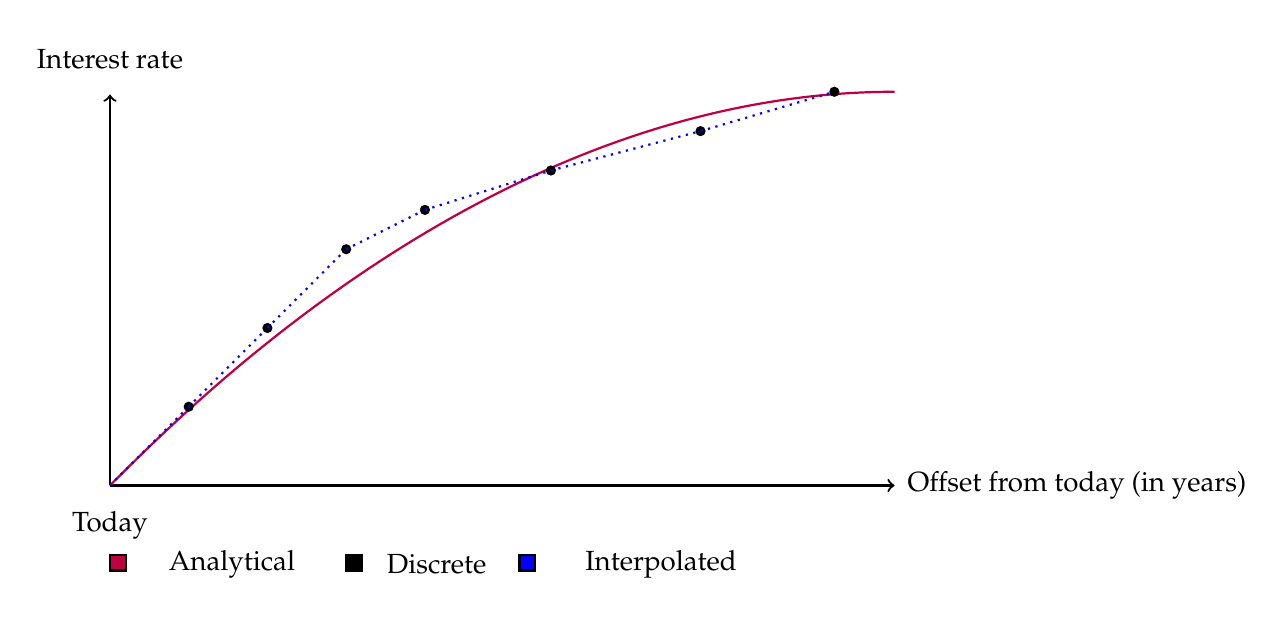
\begin{tikzpicture}[-,shorten >=1pt,auto,node distance=1.5cm,thick,minimum size=0.8cm,main node/.style={circle,draw=red,very thick}]
\tikzstyle{selected edge} = [draw,line width=6pt,-,blue!30]

\coordinate (belowstart) at (0,-1);
\coordinate (xaxis) at (10,0);
\coordinate (origo) at (0,0);
\coordinate (yaxis) at (0,5);

% Discrete points
\coordinate (d0) at (1,1);
\coordinate (d1) at (2,2);
\coordinate (d2) at (3,3);
\coordinate (d3) at (4,3.5);
\coordinate (d4) at (5.6,4);
\coordinate (d5) at (7.5,4.5);
\coordinate (d6) at (9.2,5);

% Draw axes
\draw[->] (origo) -- (xaxis) node[right] {Offset from today (in years)};
\draw[->] (origo) -- (yaxis) node[above] {Interest rate};

% Analytical
\draw[thick,draw=purple] (0,0) parabola[bend at end] (10,5);

% Discrete
\node[minimum size=2pt,draw,circle,inner sep=1pt,fill] at (d0) {};
\node[minimum size=2pt,draw,circle,inner sep=1pt,fill] at (d1) {};
\node[minimum size=2pt,draw,circle,inner sep=1pt,fill] at (d2) {};
\node[minimum size=2pt,draw,circle,inner sep=1pt,fill] at (d3) {};
\node[minimum size=2pt,draw,circle,inner sep=1pt,fill] at (d4) {};
\node[minimum size=2pt,draw,circle,inner sep=1pt,fill] at (d5) {};
\node[minimum size=2pt,draw,circle,inner sep=1pt,fill] at (d6) {};

% Linear Interpolated
\draw[dotted,draw=blue] (origo) -- (d0);
\draw[dotted,draw=blue] (d0) -- (d1);
\draw[dotted,draw=blue] (d1) -- (d2);
\draw[dotted,draw=blue] (d2) -- (d3);
\draw[dotted,draw=blue] (d3) -- (d4);
\draw[dotted,draw=blue] (d4) -- (d5);
\draw[dotted,draw=blue] (d5) -- (d6);

% Today
\node at (0,-0.5) () {Today};
% Legend
\filldraw[draw=black, fill=blue] (5.2,-1.08) rectangle node {} +(0.2,0.2);
\node at (7, -1) () {Interpolated};

\filldraw[draw=black, fill=purple] (0,-1.08) rectangle node {} +(0.2,0.2);
\node at (1.55, -1) () {Analytical};

\filldraw[draw=black, fill=black] (3,-1.08) rectangle node {} +(0.2,0.2);
\node at (4.15, -1) () {Discrete};

\end{tikzpicture}
\caption{Visualization of our term structure types.}
\label{fig:tstypes}
\end{center}
\end{figure}

The reader should note that an interest rate with offset zero (that is, today) is
always zero, since nobody would be willing to lend you money for a single day.
Due to the inverse relation of interest rates and discount factors, the discount factor
today is always 1.

Moreover, the forward rate function, \texttt{fwdRate}, is used to obtain the 
implied future zero rates. There is no conceptual leap required to understand 
these, as they are simply interest rates in the future, hence the type 
signature requiring two offsets.\\
Notwithstanding, their usefulness is may not be evident. 
Imagine three points in time, $d_0$ - today - and two
offsets in the future $d_1$ and $d_2$. We are then tasked with finding out
what the interest rate between $d_1$ and $d_2$, $R_{12}$ would be. Despite not 
knowing whether the interest rate will increase or decrease we may specify 
this by introducing \emph{arbitrage}. In brief, no arbitrage is the
assumption it is not possible to buy and sell the same good and turn a
profit i.e. "free money". Given annual rates we can now claim the following:

\begin{equation}
\underbrace{(1+R_{02})^2}_{observable} = \underbrace{(1+R_{01})}_{observable}(1 + R_{12})
\end{equation}

where $R_{xy}$ denotes the rate between two points in time $x$ and $y$. We
can now solve for $R_{12}$ to obtain the forward rate. Forward rates therefore
allow us to make statements about future interest rates as a result of the
prevailing interest rates.

% TODO more

\section{Instruments}\label{sec:instruments}

Now that we have cemented the basic theory of interest rates, discounting
and term structures we turn to their application in financial instruments.

We have defined an \texttt{Instrument} class to represent the high-level
functionality that all financial instruments must share:

%%% Explain the Instrument class %%%
\begin{hscode}
-- | Instrument is a high-level class for financial instruments
class Instrument i where
  -- | Is the instrument expired?
  expired :: i -> IO Bool
  -- | Underlying model required for pricing
  type PricingEngine :: *
  -- | Returns the present value of the instrument
  pv :: i -> PricingEngine -> IO Cash
\end{hscode}

We require an associated type to represent a pricing engine since we
cannot price all instruments in a similar fashion.\\
Due to the high-level nature of this class, very few methods qualify.
It is interesting to note that \hql defines the
exact same two functions as Quantlib's \texttt{Instrument}
class\cite{implql}. Also, Quantlib has an equivalent \texttt{PricingEngine}
class to cater for the need of different pricing methods for different
products.\\

\begin{figure}[!h]
\centering
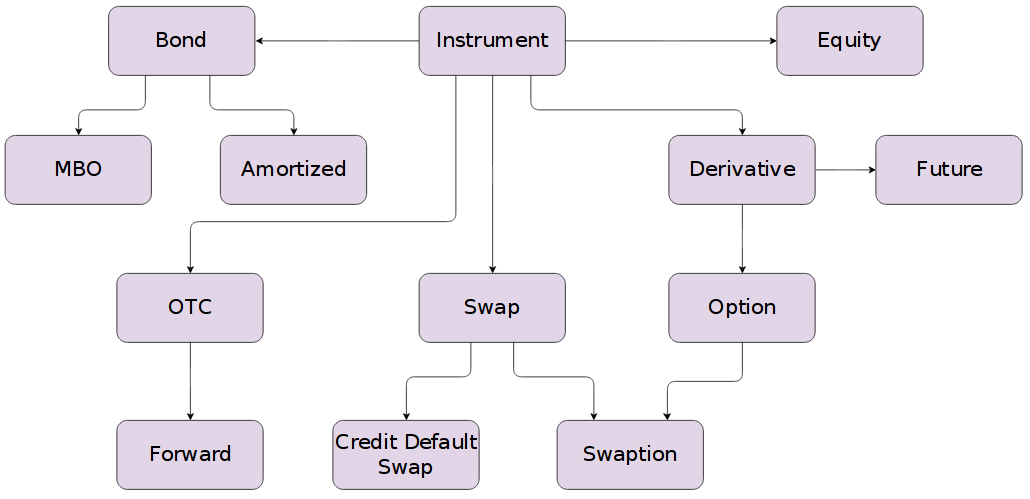
\includegraphics[scale=.3]{images/classhier.png}
\caption{Type class architecture.}
\label{fig:classhier}
\end{figure}

In the coming sections we shall delve into the specific instruments and
describe their implementations. We refer the reader to figure \ref{fig:classhier}
for and overview of the classes we have defined. The arrows denote type class
constraints e.g. a \texttt{Bond} must be an instance of \texttt{Instrument}.

\section{Fixed Income}\label{sec:fi}

In this section we will go through how we have modelled the subset of products 
in the \emph{fixed income} category, of which a product called bonds are 
the bread and butter. In brief, a bond is a financial security that promises
the bond holder a stream of future payments. These play a huge role in the 
financial markets are are typically only offered by governments or large 
financial institutions.\\
We will present our \texttt{FixedIncome} module by means of a running example
of a bond. A \emph{serial} is an example of a bond that equates to a typical 
Danish house loan. The cash flow of the holder of a 5 year serial with annual 
repayments is depicted in figure \ref{fig:serialcf}.\\

\begin{figure}[!h]
\begin{center}
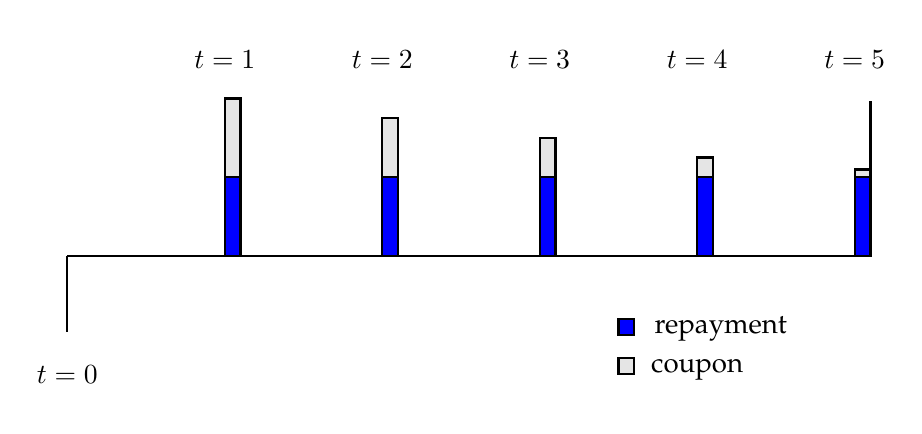
\begin{tikzpicture}[-,shorten >=1pt,auto,node distance=1.5cm,thick,minimum size=0.8cm,main node/.style={circle,draw=red,very thick}]
\tikzstyle{selected edge} = [draw,line width=6pt,-,blue!30]

\coordinate (belowstart) at (0,-1);
\coordinate (start) at (0,0);
\coordinate (stop) at (10.2,0);
\coordinate (abovestop) at (10.2,2);
\draw (start) -- (stop);
\draw (start) -- (belowstart);
\draw (stop) -- (abovestop);

\node at (0, -1.5) () {$t=0$};

\filldraw[draw=black, fill=blue] (2,0) rectangle node {} +(0.2,1);
\filldraw[draw=black, fill=lightgray]  (2,1) rectangle node {} +(0.2,1);
\node at (2, 2.5) () {$t=1$};

\filldraw[draw=black, fill=blue] (4,0) rectangle node {} +(0.2,1);
\filldraw[draw=black, fill=lightgray]  (4,1) rectangle node {} +(0.2,0.75);
\node at (4, 2.5) () {$t=2$};

\filldraw[draw=black, fill=blue] (6,0) rectangle node {} +(0.2,1);
\filldraw[draw=black, fill=lightgray]  (6,1) rectangle node {} +(0.2,0.5);
\node at (6, 2.5) () {$t=3$};

\filldraw[draw=black, fill=blue] (8,0) rectangle node {} +(0.2,1);
\filldraw[draw=black, fill=lightgray]  (8,1) rectangle node {} +(0.2,0.25);
\node at (8, 2.5) () {$t=4$};

\filldraw[draw=black, fill=blue] (10,0) rectangle node {} +(0.2,1);
\filldraw[draw=black, fill=lightgray]  (10,1) rectangle node {} +(0.2,0.1);
\node at (10, 2.5) () {$t=5$};

% Legend
\filldraw[draw=black, fill=blue] (7,-1) rectangle node {} +(0.2,0.2);
\node at (8.3, -0.92) () {repayment};

\filldraw[draw=black, fill=lightgray] (7,-1.5) rectangle node {} +(0.2,0.2);
\node at (8, -1.44) () {coupon};

\end{tikzpicture}
\caption{Cashflow of a serial.}
\label{fig:serialcf}
\end{center}
\end{figure}

We observe that the bond issuer makes fixed size deposits to the counterpart to 
repay the loan. Since there is no such thing as a free lunch, so-called coupon 
payments are made in addition to compensate for having its funds tied up. These
payments are simply the bond's interest rate applied to the face value of the
bond, and are decreasing as a result of the repayment amortization\cite{hqldoc}.\\

In addition to the serial, we present the most basic bond imaginable, the zero 
coupon bond or simply \emph{zero}. It is exactly that - a bond with a specified 
tenor and interest rate that pays a fixed amount at maturity.\\

We have designed a class to encapsulate the functionality of bonds:

%%% Explain the Bond class %%%
\begin{hscode}
type Payment = (Date,Cash) -- A payment is cash on some date
type Payments = [Payment]
-- | Bond class specifies common denominator for all bond types 
class Instrument b => Bond b where
  -- | Returns dirty price on a given date
  dirty :: TermStructure ts => b -> ts -> Date -> Cash
  -- | Principal (or face value) of a bond
  principal    :: b -> Cash
  -- | A list of Payments indicating remaining cashflow
  outstanding  :: b -> Payments
  -- | Returns a list of Payments representing the cashflow
  -- over the bond over its lifetime
  cashflow     :: b -> Payments
  -- | Returns the coupon part of the cashflow
  coupons      :: b -> Payments
  -- | Returns the dates at which cashflow is exchanged
  paymentDates :: b -> [Date]
\end{hscode}

The \texttt{cashflow} function generates a list of payments exactly as shown
in figure \ref{fig:serialcf} while \texttt{coupons} generates only the coupon
payments.
A serial is an example of an \emph{amortized} bond, meaning that the writer
of a serial (the person who initially lended the money) receives repayments over
the lifetime of a bond. As these loan-based bonds come in multiple flavours
we have therefore created an \texttt{Amortized} class:

\begin{hscode}
-- | Class declaration for amortized bonds
class Bond a => Amortized a where
  repayments :: a -> Payments
\end{hscode}

allowing users to retrieve a list of payments representing the coupon payment
subtracted from the cashflow. \texttt{repayments} now generate the blue repayment part of the cashflow
we observe in figure \ref{fig:serialcf}.\\

Returning to our serial example, we have defined a data type for fixed coupon
amortized bonds using a Haskell generalized algebraic data type (GADT):

\begin{hscode}
data FixedAmortizedBond where 
  Annuity :: { asett :: Date,
               amatu :: Date,
               aface :: Cash,
               arate :: Double,
               astms :: Settlements,
               adcc  :: (DayCount d) => d,
               aroll :: RollConvention } -> FixedAmortizedBond
  Serial :: {  asett :: Date,
               amatu :: Date,
               aface :: Cash,
               arate :: Double,
               astms :: Settlements,
               adcc  :: (DayCount d) => d,
               aroll :: RollConvention } -> FixedAmortizedBond
\end{hscode}

where the fields are explained in table \ref{tab:fields}.

\begin{center}  
\begin{longtable}{l|l|l}
Field & Meaning & Usage\\\hline
\texttt{asett} & Settlement date & Start date for interpolation\\
\texttt{amatu} & Maturity date & End date for interpolation\\
\texttt{aface} & Face Value & Used to compute repayment and coupons\\
\texttt{astms} & Settlements per Year & Used to generate payment dates\\
\texttt{adcc} & Daycount convention & Used in discounting\\
\texttt{aroll} & Roll convention & Resolves illegal payment dates (e.g. weekends)\\
\caption{\texttt{FixedAmortizedBond} fields}
\end{longtable}
\label{tab:fields}
\end{center}

Note that although the \texttt{Annuity} loan has the same fields as our serial,
we need a separate constructor for it as the cashflow generation is completely
different for this bond type\cite{hqldoc}. In addition to the zero and amortized
bonds, \hql also feature a consol and bullet bond. We refer to appendix?

%%% Haskell %%%
A central tenet of our architecture is that we keep the backend
as simple as possible and keep the interface detailed and 
self-explanatory. This way we keep the mathematical formulas as transparent
and clean as possible while the interface remains user-friendly.\\

The backend for pricing bonds exploits the fact that all instances must define
the \texttt{cashflow} function. As we saw in section \ref{sec:discounting},
pricing a cashflow is simply multiplication by a discount factor. This means
that pricing a bond $b$ can be formulated as follows:

\begin{equation}
PV_b = \sum_{k=0}^n df_k cf_k
\end{equation}

where $cf_k$ and $df_k$ denote a cashflow or discount factor at time $k$,
respectively. As a result, the backend for bond pricing is implemented as:

\begin{hscode}
pv = sum $ zipWith (*) cashflowList discountFactors
\end{hscode}

\section{Options, Futures and other Derivatives}

In this section we briefly describe how our architecture caters to other
financial products in addition to the fixed income instruments we have seen.\\

In figure \ref{fig:classhier} we defined the inheritance relations that
exist in terms of financial products and how we are to model them using 
Haskell's class system. \hql currently implements the toolbox required
for the implementation of the resulting products. The only constraint on
new additions to \hql is the \texttt{Instrument} class which all products
must be an instance. This means that the challenge lies the the fact
that we must define an appropriate \texttt{PricingEngine} type for each
class of products.\\

A \emph{call option} is a contract that gives the holder the right to purchase
(or \emph{exercise} a good or service (this is called the \emph{underlying}) 
at a specific price (the \emph{strike}). What pricing engine is appropriate 
for such a contract; does it depend on the underlying?
In fixed income we saw that the term structure of interest rates qualified,
but this is not the case for options.

Instead, we may want to use a Black-Scholes model for European
options\cite{cmunk} or a binomial model for American\footnote{The distinction
between American and European has nothing to do with geography. European
options may only be exercised at maturity, while American ones can be
exercised at any time.} options.

While it is possible to price European-style options using a closed-form 
solution, we must apply simulation methods to price the American counterpart.\\
The associated type, \texttt{PricingEngine} is therefore liberal enough to
allow us to specify something like:

\begin{hscode}
-- European options
newtype BlackScholes = (EuropeanOption -> Cash)
instance Instrument EuropeanOption where
  type PricingEngine = BlackScholes

-- American options
instance Instrument EuropeanOption where
  type PricingEngine = BinomialModel
\end{hscode}
\ab{Still working on this}

%First of all, a natural next step in the development of HQL is the 
%implementation of derivatives which is itself a product relying on another- the 
%\emph{underlying} - hence the the name. An example of this is 
%a forward-rate agreement, the simplest being an agreement where two parties 
%agree on a future trade of a commodity. It should be obvious that the price of 
%the underlying directly affects the value of having entered such an agreement.\\
%
%However, with the addition of floating rate bonds, we may model fixed income 
%derivatives such as swaps. A swap is contract in which two counterparties agree 
%to exchange two cashflows.

%Fixed
%Floating
%Fixed
%Inter-currency
%Vanilla
%Floating
%Vanilla

%There are two obvious ways in which we can extend HQL with interest rate 
%derivatives support. For instance, swaps can be modelled by combining a fixed 
%and a floating leg, the latter still not yet being supported. On the other 
%hand, it could be built as a list of forward-rate agreements (make sure this is 
%explained above, or refer to Appendix) between the two parties in question.

\chapter{Results}

\section{Evaluation}

\section{Architecture}

\section{Performance}

\section{Precision and Symbolic Computations}

\chapter{Future Work}\label{chap:fw}

Our project is far from a fully-fledged library, and many more modules must be added.

First of all we do not have support for the floating rate bonds
(see appendix X section something) due to the lack of of Monte Carlo
simulation module. A natural next step after floating rate support
would then be to implement interest rate derivatives such as swaps.

There are two obvious ways in which we can extend HQL with interest rate
derivatives support. For instance, swaps can be modelled by combining a
fixed and a floating leg, the latter still not yet being supported. On the
other hand, it could be built as a list of forward-rate agreements (make sure
this is explained above, or refer to Appendix) between the two parties in
question.\\

Alas, our library is also missing a key component which is a proper calendar
module. We currently allow the users to supply a variable number of
settlements per year. This needs to be constrained so that the users either
specify a standard settlement pattern (missing an example) or \emph{all}
payment dates for OTC products. Moreover, HQL currently assumes that all
weekdays are valid payments dates. This doesn't cater to local holidays
(e.g. January $1^{\text{st}}$ in Denmark, $4^{\text{th}}$ of July in the
United States, etc) which may be computed as offsets from Easter Sunday.\\

Another interesting extension is to implement a way of generating term
sructures from portfolios using bootstrapping and interpolation\footnote{need
a reference to Björk/Munk here}. This would essentially allow users to import
data from external sources and use HQL to build term structures and perform
bond valuation.\\

Support for mortgage-backed bonds is also missing in our library. We provide
an MBO class to be used in the future.\\
%Prepayment estimates must also be computed.

%Cubic splines or Nelson-Siegel method for obtain term structure as a function.

Finally, it would be desirable to implement an embedded domain-specific language
for construction of over-the-counter (OTC) products.
As OTC products are subject to counterparty risk, this would be another topic
to investigate.

%The class hierarchichy should be extended to define interfaces for derivatives,
%commodities, money markets etc.. Draw diagram?

\chapter{Conclusion}


%\printglossary

\newglossaryentry{computer}
{
  name=computer,
    description={is a programmable machine that receives input,
                   stores and manipulates data, and provides
                                  output in a useful format}
}

%-----------------------------------------------------------

%\printglossary[type=\acronymtype,title={List of Abbreviations},toctitle={List of Abbreviations}]
\addcontentsline{toc}{chapter}{\numberline{}Bibliography}
\bibliographystyle{plain}
\bibliography{hql}

\printglossary[type=main,title={Glossary},toctitle={Glossary}]
%In this section the terminology used in the field of fixed income and how it applies to HQL.
%\thispagestyle{empty}
%\cleardoublepage
%\printglossary[type=\acronymtype,title={List of Abbreviations},toctitle={List of Abbreviations}]

\printindex


%-----------------------------------------------------------
\appendix

\chapter{Contributions}

\newcounter{treeline}

\newcommand{\treeroot}[1]{% Title
\node[above] at (0,0) {#1};%
\setcounter{treeline}{0}
}

\newcommand{\treeentry}[2]{% Title, Level
\draw[->] (#2-1,-\value{treeline}/2) -- (#2-1,-\value{treeline}/2-0.5) -- (#2+0.5,-\value{treeline}/2-0.5) node[right] {#1};
\stepcounter{treeline}
}

\newcommand{\altentry}[2]{% Title, Level
\draw[->] (#2-1,-\value{treeline}/2) -- (#2-1,-\value{treeline}/2-0.5) -- (#2+0.5,-\value{treeline}/2-0.5) node[right] {#1};
\foreach \x in {1,...,#2}
{   \draw (\x-1,-\value{treeline}/2) -- (\x-1,-\value{treeline}/2-0.5);
}
\stepcounter{treeline}
}

\textcolor{blue}{Andreas Bock}\\
\textcolor{green}{Johan Astborg}\\
\textcolor{red}{Both}\\

\begin{tikzpicture}
\tt
\treeroot{src}
\treeentry{Instruments}{1}
\treeentry{\color{blue} Instrument.hs}{2}
\treeentry{FixedIncome}{2}
\treeentry{Bonds}{3}
\treeentry{\color{blue} Bonds.hs}{4}
\treeentry{Utils}{2}
\treeentry{\color{green} InterestRate.hs}{2}
\treeentry{\color{red} TermStructure.hs}{2}
\treeentry{Derivatives}{2}
\treeentry{\color{blue} Derivatives.hs}{3}
\treeentry{Equity}{2}
\treeentry{OTC}{2}

\treeentry{Pricing}{1}
\treeentry{Utils}{1}
\treeentry{\color{blue} Calendar.hs}{2}
\treeentry{\color{red} Currency.hs}{2}
\treeentry{\color{blue} DayCount.hs}{2}
\treeentry{Graphics}{2}
\treeentry{\color{green} Visualize.hs}{3}
\end{tikzpicture}




%-----------------------------------------------------------
\end{document}
